We trained a simple fully connected neural network on the keypoint data gathered in Q1.1, and used this model to classify poses.
The model was trained on 400 hand classified samples (even split game, movie) of our 40,000+ total samples.
Our model achieved $90\%$ accuracy, after 2 hours of training, on our test set of 100 samples.
The failures of this model were often acceptable, owing to the non-distinct nature of the 5 classes (where does half a body end and a head begin?).
There were far fewer unacceptable errors, thus this method proved effective for its simplicity (see Figure \ref{fig:Q1_2}).

\begin{figure}[h!]
  \begin{center}
  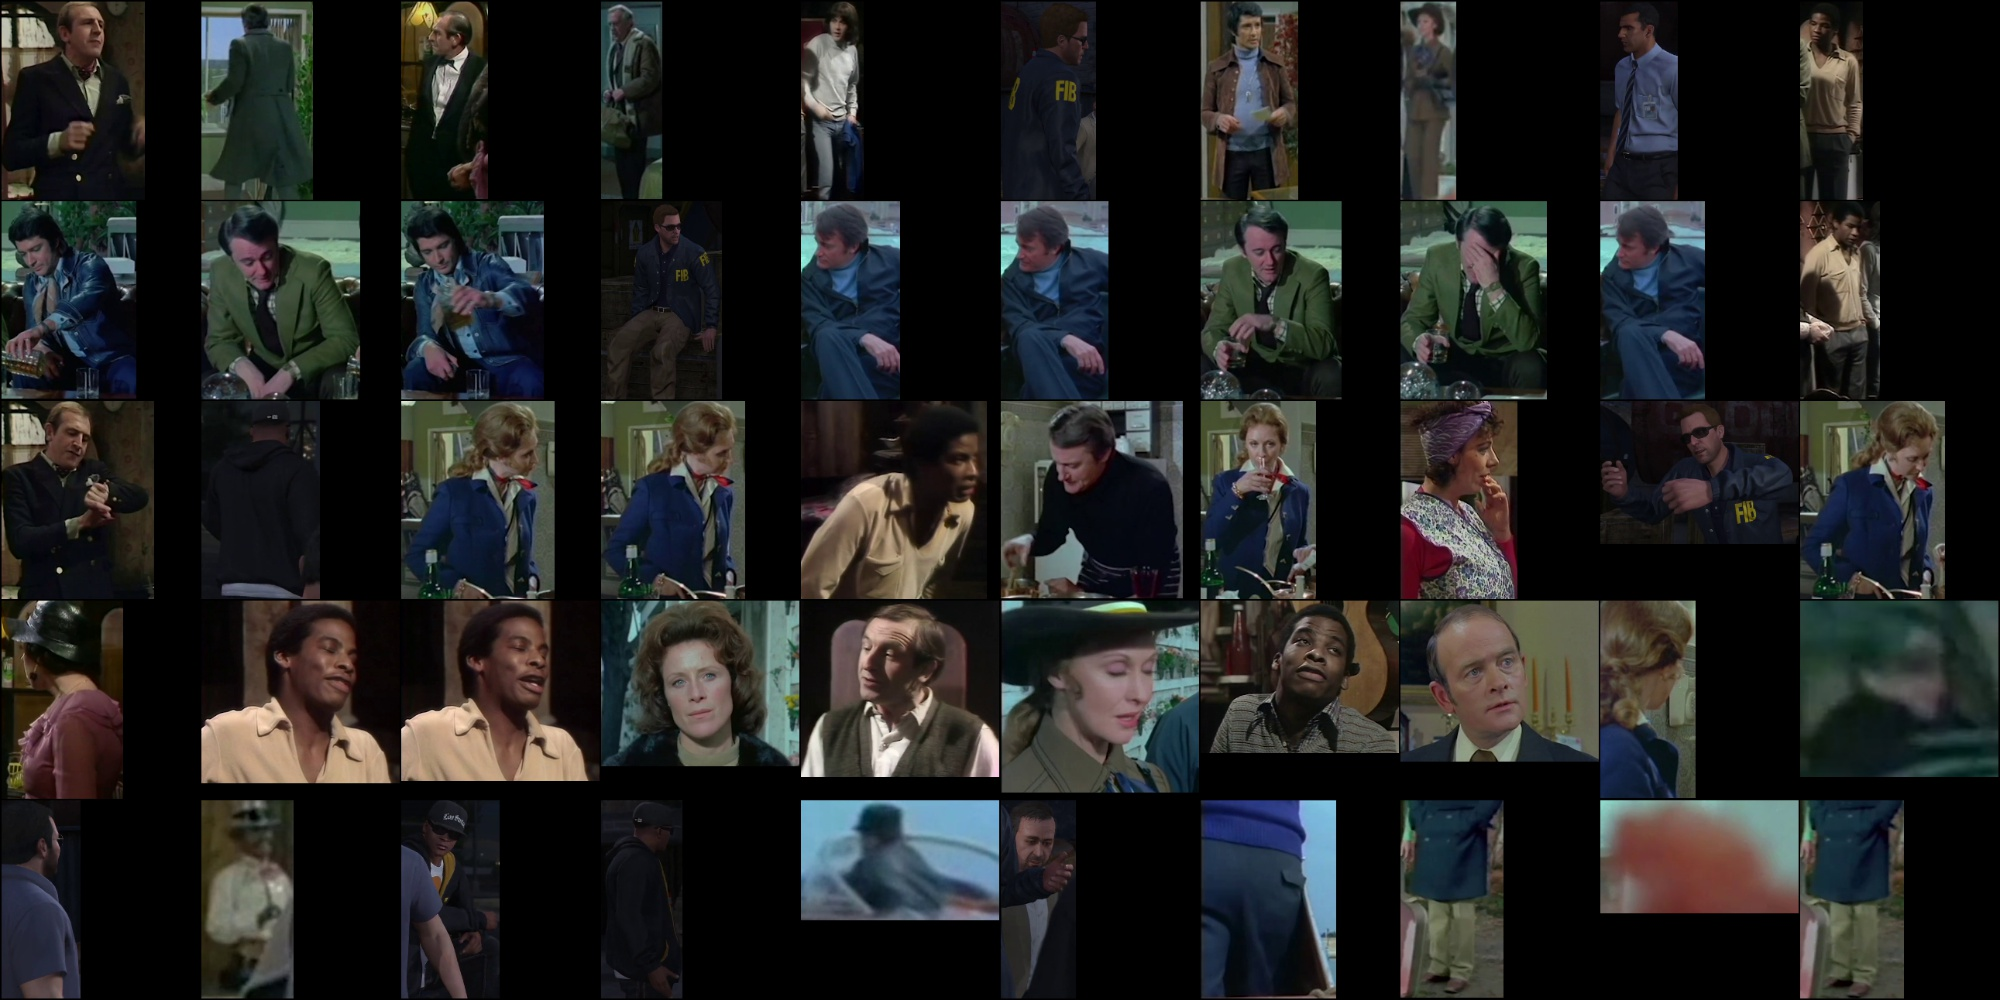
\includegraphics[scale=0.2]{Q1_2_full.jpg}
    \caption{Q1.2 sample classified human patches. From top to bottom each row is class: full-body, sitting, half-body, head, other.}
    \label{fig:Q1_2}
  \end{center}
  \end{figure}